%
% File naaclhlt2018.tex
%
%% Based on the style files for NAACL-HLT 2018, which were
%% Based on the style files for ACL-2015, with some improvements
%%  taken from the NAACL-2016 style
%% Based on the style files for ACL-2014, which were, in turn,
%% based on ACL-2013, ACL-2012, ACL-2011, ACL-2010, ACL-IJCNLP-2009,
%% EACL-2009, IJCNLP-2008...
%% Based on the style files for EACL 2006 by 
%%e.agirre@ehu.es or Sergi.Balari@uab.es
%% and that of ACL 08 by Joakim Nivre and Noah Smith

\documentclass[11pt,a4paper]{article}
\usepackage[hyperref]{naaclhlt2018}
\usepackage{times}
\usepackage{latexsym}
\usepackage{multirow}
\usepackage{url}
\usepackage{amssymb}
\usepackage{amsmath}
\usepackage{hyperref}
\usepackage{algorithm}
\usepackage{algpseudocode}
\usepackage{graphicx}
\newcommand{\argmin}[1]{\underset{#1}{\operatorname{argmin}}\;}
\newcommand{\argmax}[1]{\underset{#1}{\operatorname{argmax}}\;}
\aclfinalcopy % Uncomment this line for the final submission
\def\aclpaperid{434} %  Enter the acl Paper ID here

%\setlength\titlebox{5cm}
% You can expand the titlebox if you need extra space
% to show all the authors. Please do not make the titlebox
% smaller than 5cm (the original size); we will check this
% in the camera-ready version and ask you to change it back.

\newcommand\BibTeX{B{\sc ib}\TeX}

\title{Toward Featureless Event Coreference Resolution via Conjoined Convolutional Neural Networks}

\author{Chris Tanner \textnormal{and} Eugene Charniak\\
Brown Linguistic Laboratory of Information Processing \\
  Brown University \\
  Providence, RI  02912 \\
  {\tt \{christanner,ec\}@cs.brown.edu} \\}

\date{}

\begin{document}
\maketitle
\begin{abstract}
% motivation / others' weaknesses
Coreference resolution systems for entities and/or events almost always make use of many linguistic, parsing-based features.  In contrast, (1) we introduce a new state-of-the-art event coreference resolution system which uses only lemmatization and its corresponding precomputed word embeddings, achieving 66.9 CoNLL F1 score on a common ECB+ test set, along with setting a new baseline of 81.2 for the test set at large. (2) We exhaustively illustrate the performance of other commonly-used features.  The crux of our system is that it first makes pairwise event-coreference predictions by using a Conjoined Convolutional Neural Network.  Last, (3) we cluster the event mentions with a simple, but novel, neural approach which performs merges in an easy-first, cluster-holistic manner, allowing our system to be less susceptible to errors that are made exclusively from min-pairwise decisions.
\end{abstract}

\section{Introduction}
% problem definition/statement
Coreference resolution is the task of trying to identify -- within a single text or across multiple documents -- which \textit{mentions} refer to the same underlying discourse \textit{entity} or \textit{event}.  A \textit{mention} is defined as a particular instance of word(s) in a document (e.g., \textit{she} or \textit{announced}).  Ultimately, coreference resolution is a clustering task, whereby we wish to group all like-mentions together, as shown in Figure \ref{fig:corpus}.  Successfully doing so can be useful for several other core NLP tasks that concern natural language understanding, such as information extraction \cite{Humphreys:1997}, topic detection \cite{Allan:1998}, text summarization \cite{Daniel:2003}, knowledge base population \cite{Cross_Document_Coreference_Resolution_A_Key_Technology_for_Learning_by_Reading}, question answering \cite{Narayanan:2004:QAB:1220355.1220455}, etc.

\begin{figure}[ht]
\centering
	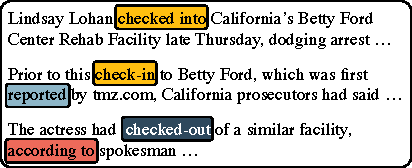
\includegraphics[width=0.45\textwidth]{corpus}
	\caption{Sample of the ECB+ corpus, depicting gold coref mentions as having shared box colors.}
	\label{fig:corpus}
\end{figure}

% problem definition
Specifically, coreference systems aim to find a globally-optimal fit of mentions to clusters, whereby every mention $m$ in the corpus is assigned to exactly one cluster $C$, the membership of which constitutes that every ${m_i,m_j} \in C_k$ is co-referent with each other.  If a given $m_i$ is not anaphoric with any other $m_j$, then it should belong to its own $C_k$ with a membership of one.  Further, the number of distinct clusters is not known apriori, and it is implicitly the responsibility of the system to determine.  Finding a globally-optimal assignment of clusters is NP-Hard and thus computationally intractable.  In attempt to avoid this, systems typically perform pairwise-mention predictions, then use those predictions to build clusters. The specific modelling strategies for such approximately fall into two categories: (1) mention-ranking / mention-pairs; and (2) entity-level / event-level.

\textbf{Mention-ranking} models define a scoring function $f(m_i,m_j)$ which operates on a mention $m_j$ and possible antecedent $m_i$, where $m_i$ occurs earlier in the document and could be null (represented by $\epsilon$ and denoting that $m_j$ is non-anaphoric).  Wiseman, et. al.'s \shortcite{DBLP:journals/corr/WisemanRS16} strong model is an example.

\textbf{Mention-pair} models are defined almost identically to mention-ranking ones, with the subtle difference being the target objective of the pairwise-candidates.  That is, mention-ranking model aim to find the ideal $m_i$ antecedent for every $m_j$, whereas mention-pair models score all possible $(m_i,m_j)$ pairs.  Because these models base their predictions on the information from just two mentions at a time, they are by definition less expressive than entity/event-level models.  However, their inference can be relatively simple and effective, allowing them to be fast and scalable.  Consequently, they have often been the approach used by many state-of-the-art systems \cite{Soon:2001:MLA:972597.972602,DBLP:conf/emnlp/DurrettK13}.

\textbf{Entity/Event-level} models differ in that they focus on building a global representation of each underlying entity or event, the basis of which determines each mention's membership -- as opposed to operating on a mention-level basis \cite{DBLP:journals/corr/WisemanRS16,clark2016improving}.

In this work, we use a novel mention-pair model that is designed to discriminate between pairs of input features: Siamese Convolutional Neural Networks.  We feel awkward using the term ``siamese,'' so we will henceforth refer to our model as our newly-coined term, Conjoined Convolutional Neural Networks (or CCNN).  Further, we aim to replace a common weakness of mention-pair models with an approach resembling the main strength of entity/event-level models. Specifically, we aim to combine all linked mention pairs into a cluster via a neural, easy-first clustering approach which factors in a small, but effective, notion of the entire cluster at large.

Additionally, coreference research systems typically use a plethora of relatively expensive parsing-based features, including dependency parse information, lemmatization, WordNet hypernyms/synonyms, FrameNet semantic roles, etc.  Although some research papers list their system's learned feature weights \cite{journals/tacl/YangCF15}, there has been a striking lack of work which takes the minimalist approach and illustrates the effects of using few features.  We aim to address this by starting with a basic lemma-embedding feature and then evaluate the effectiveness of adding other commonly used features.

Finally, in general, \textit{event} coreference resolution has received drastically less attention than \textit{entity} coreference.  However, in this paper, we are exclusively interested in within-doc event coreference.

In summary, we introduce a novel mention-pair approach to event coreference resolution by using a Conjoined Convolutional Neural Network and unusually few features.  We contribute detailed results of other commonly used features.  And last, we combine our predicted mention pairs into clusters via a simple neural approach which attempts to represent each cluster as a whole, yielding state-of-the-art results on the ECB+ corpus.


% the problem
%In this paper,   Further, we wish to address the possible shortcoming of 
%Again, the main shortcoming of the two former mention-* models is that after making pairwise decisions, combining them into clusters only requires satisfying local constraints
% our solution
% explain subsequent chapters

\section{Related Work}
% initial start
The seminal research on event coreference can be traced back to the DARPA-initiated MUC conferences, whereby the focus was on limited scenarios involving terrorist attacks, plane crashes, management succession, resignation, etc. \cite{Humphreys:1997,Bagga:1999:CEC:1608810.1608812}.


%Event coreference resolution has received significantly less attention than its entity-based counterpart.  The seminal research on event-based coreference can be traced back to the DARPA-initiated MUC conferences, whereby the focus was on limited scenarios involving terrorist attacks, plane crashes, management succession, resignation, etc.  Most notable from this period were the works by Humphreys et al. \shortcite{Humphreys:1997} and Bagga and Baldwin \shortcite{Bagga:1999:CEC:1608810.1608812}, which applied event coreference to the tasks of information extraction, topic detection and tracking.

% continued efforts
%The successor of MUC was the annual ACE program, which occurred from 1999 to 2008 and furthered researched by including corpora containing more fine-grained events.  This addressed the aforementioned challenge whereby events may be an overloaded term in that multiple, uniquely distinct underlying events may use textually-identical mention representation.  One of the most notable papers from this period, which also illustrates the varied modelling approaches, is the graph-based system by Chen and Ji \shortcite{Chen:2010:GCC:1870490.1870491}.  This is an example of a mention-pair model, as they constructed a graph from the fully-complete weight matrix that corresponds to all mention pairs.

In the present day, Deep Learning is revolutionarily affecting NLP; however, there has been only a few successful applications of deep learning to coreference resolution, almost all of which have been for \textit{entity} coreference.  We attribute this dearth to the fact that coreference resolution is inherently a clustering task, which tends to be a non-obvious modality for deep learning.  Since our model (1) uses deep learning and (2) operates on the ECB+ corpus, we organize the related research into the following categories:

\subsection{Deep Learning Approaches}
To the best of our knowledge, there are only five publications which apply deep learning to coreference resolution, four of which focus on entity coreference.

Sam Wiseman, et. al. \shortcite{DBLP:conf/acl/WisemanRSW15,DBLP:conf/naacl/WisemanRS16} trained a mention-ranking model with a heuristic loss function that assigns different costs based on the types of errors made, and their latter work used mention-ranking predictions towards an entity-level model.
Clark and Manning \shortcite{clark2016improving,DBLP:journals/corr/ClarkM16a} also built both a mention-ranking model and an entity-level model, the former of which was novel in using reinforcement learning to find the optimal loss values for the same four distinct error types defined in Wiseman's, et. al. \shortcite{DBLP:conf/acl/WisemanRSW15} work.

\subsection{Systems using ECB+ Corpus}
% most related
For our research, we make use of the ECB+ corpus \cite{ECB+}, which we further describe in Section \ref{sec:corpus}.  This rich corpus provides annotations for both entities and events, yet most research chooses to focus on using \textit{either} events \textit{or} entities, not both.  To the best of our knowledge, there are only two papers which focus on the event mentions of ECB+: The Hierarchical Distance-dependent Chinese Restaurant Process (HDDCRP) model by Yang, et. al. \shortcite{journals/tacl/YangCF15} and Choubey's and Huang's Iteratively-Unfolding approach \shortcite{Choubey2017EventCR}.

\subsubsection{HDDCRP Model}
\label{sec:HDDCRP}
% HDDCRP
Yang, et. al's HDDCRP model \shortcite{journals/tacl/YangCF15} uses a clever mention-pair approach, whereby they first use logistic regression to train parameters $\theta$ for the similarity function in Equation \ref{eq:hddcrp}.  
\begin{equation}
\label{eq:hddcrp}
f_{\theta}(x_i,x_j) \propto \textnormal{exp\{} \theta^T\psi(m_i,m_j)\textnormal{\}}
\end{equation}
Then, in a Chinese-restaurant-process fashion, they probabilistically link together mentions based purely on the scores provided by this similarity function.  That is, the value of $f(m_i,m_j)$ is directly correlated with the probability of $(m_i,m_j)$ being chosen as a linked pair.  Then, identical to Bengtson's and Roth's work \cite{Bengtson:2008:UVF:1613715.1613756}, the HDDCRP model forms clusters by tracing through all linked pairs. All mentions that are reachable by a continuous path become assigned the same cluster.  This hinges on the transitive property of coreference.  For example, if ${(m_1,m_3),(m_3,m_5)}$ and $(m_5,m_6)$ are each individually linked via the scoring function, then a cluster $C_i$ is formed, where $C_i = \{m_1,m_3,m_5,m_6\}$, even though $(m_1,m_5)$ or $(m_3,m_6)$ may have had very low similarity scores. We aim to improve this shortcoming, as detailed in Section \ref{sec:clustering}.

\subsubsection{Neural Iteratively-Unfolding Model}
\label{sec:Choubey}
% Choubey
Recently, Choubey and Huang \shortcite{Choubey2017EventCR} introduced the first neural model for event coreference.  Their system also fits into the mention-pair paradigm, whereby mentions are predicted by a feed-forward neural network. Their within-doc model's features are based on the cosine similarity and Euclidean distance of input-pair embeddings.  Their cross-document model is identical, but with context embeddings added to the input.  The authors asserted that when using the ECB+ corpus, within-doc coreference did not benefit from using mention context, which is an important finding.  However, similar to the weakness of the HDDCRP model, they merge clusters which contain \textit{any} mention-pair whose predicted score is below a given threshold, independent of mentions' relation to the cluster at large.

\section{System Overview}
\subsection{Mention Identification}
\label{sec:mentionid}
Coreference systems are predicated upon having entity/event mentions identified.  In fact, this identification process is the focus of a different line of research: entity recognition and event detection.  This separation of tasks allows coreference systems to be evaluated precisely on their ability to cluster together appropriate mentions, independent from the mention detection.  Thus, it is common practice for coreference systems to either: (1) use gold mentions that are defined by the true annotations in the corpus, or (2) use an off-the-shelf entity recognition system.  We do both; the majority of our results are shown using gold ECB+ test mentions.  Yet, to ensure we developed a competitive system, we also used the same test mentions as the HDDCRP and Iterative-Unfolding models.

The HDDCRP model used a pre-existing event detection system to identify mentions, then they filtered many of those, yielding their system with an imperfect but reasonable set of mentions that shares a moderate overlap with the gold test mentions.  Determining the exact mentions that were used by HDDCRP was one of the most challenging and time-consuming processes of our research.

The Iteratively-Unfolding system also aimed to test on the HDDCRP predicted mentions.  After numerous exchanges with the author, it was clear that their set of mentions was similar and reasonable for research, but understandably not the same as that used by HDDCRP.  Namely, they filtered out: (1) all predicted mentions which were not in the gold set (false positives), and (2) predicted mentions which were singletons (ones that did not cluster with a mention from another document).

We evaluate our systems having used the: (1) gold mentions; (2) HDDCRP-predicted mentions; (3) Iteratively-Unfolding-predicted mentioned.

\subsection{Reproducibility}
We provide our code online,\footnote{\url{WILL_INSERT_GITHUB_LINK}} which is written in Keras \cite{chollet2015} and is easily runnable on any of the aforementioned sets of mentions and evaluations.  Additionally, our code runs in just a few minutes on a single Titan X GPU.
\subsection{Models}
Our system is comprised of two neural models:
\begin{itemize}
  \item Conjoined Convolutional Neural Network -- used for making mention-pair predictions.  (Section \ref{sec:CCNN})
  \item Neural Clustering -- uses the pairwise predictions to cluster mentions into events (Section \ref{sec:clustering})
\end{itemize}
\subsection{Corpus}
\label{sec:corpus}
We use the ECB+ corpus \cite{ECB+}, which is the largest available dataset with annotations for event coreference.  The corpus is comprised of 43 distinct \textit{topics} -- categories or news stories -- each of which has 2 sub-topics which are similar in nature but distinctly different from each other.  For example, Topic 1 contains two sub-topics: one about Lindsay Lohan checking into a rehab center, the other about Tara Reid doing so.  Each sub-topic contains roughly 10 short text documents which all concern the same given sub-topic.  We maintained the same train/dev/test splits as previous researchers.\footnote{Training set contains topics 1-20, the Dev set contains topics 21-23, and the Test set has topics 24-43.}  A sample of the corpus in shown in Figure \ref{fig:corpus}, and statistics are listed in Table \ref{tab:ECB1}, where it is clear that the majority of gold mentions are one token in length (e.g, \textit{announced}).

\begin{table}
\centering
\begin{tabular}{c|c|c|c|c|}
\cline{2-5}
& Train & Dev & Test & Total \\ \cline{1-5} \hline
\multicolumn{1}{ |c| }{\# Documents} & 462 & 73 & 447 & 982   \\ %\cline{1-5}
\multicolumn{1}{ |c| }{\# Sentences} & 7,294 & 649 & 7,867 & 15,810    \\ 
%\multicolumn{1}{|c|}{\multirow{2}{*}{\pbox{2cm}{Mention\\length}}} & & & & \\ 
\multicolumn{1}{ |c| }{\# Mentions-1} & 1,938 & 386 & 2,837 & 5,161    \\ %\cline{1-5}
\multicolumn{1}{ |c| }{\# Mentions-2} & 142 & 52 & 240 & 434    \\ %\cline{1-5}
\multicolumn{1}{ |c| }{\# Mentions-3} & 18 & -- & 25 & 43    \\% \cline{1-5}
\multicolumn{1}{ |c| }{\# Mentions-4} & 6 & -- & 7 & 13   \\ \cline{1-5}
\end{tabular}
\caption{Statistics of the ECB+ Corpus, where Mentions-N represents event mentions which are N-tokens in length.}
\label{tab:ECB1}
\end{table}

\section{Conjoined Convolutional Neural Network}
\label{sec:CCNN}
\subsection{Motivation}
In the training data, the mentions that belong to the same gold cluster often have little variance amongst their text.  This, coupled with Choubey's, et. al. \shortcite{Choubey2017EventCR} conclusion that context does not improve within-doc performance for our corpus, lends us to believe that an event-level model would be unnecessary and probably worse than a mention-pair model.  Thus, we continue the trend of using a mention-pair model for event within-doc coreference.

\subsection{Overview}
Conjoined Neural Networks (a.k.a. Siamese Networks) were first introduced by Bromly and LeCun \shortcite{SiameseNet} for the task of determining if two input items (hand signatures) were from the same person or not.  Specifically, a Conjoined Network can be defined as two identical neural networks, each of which accepts distinct inputs, which are joined by a single loss function over their highest-level features.  The loss function computes a similarity score (e.g., euclidean distance) for an input pair.  The two networks are said to be conjoined because they share the same weights and thus work together as one network that learns how to discriminate.  The benefits of tying the weights are that it: (1) ensures that similar inputs will be mapped appropriately, otherwise, they could be mapped to hidden representations that are disproportionately dissimilar from their input representations; and (2) forces the network to be symmetric.  Namely, if we were to abstractly view the Conjoined Network as a function, then:

\vspace{4mm}

 $CCNN(f_i,f_j) \equiv CCNN(f_j,f_i)$

\vspace{4mm}

This is critical, as the CCNN's similarity function should be independent of the ordering of its input pair.

Last, CCNN's have been shown to perform well in low-resource situation \cite{Koch2015SiameseNN}.  This is ideal for our task, as it is highly likely that at test time we will encounter event mentions that are OOV.  We desire our model to discriminately learn the relationships of input mentions, rather than exclusively relying on and memorizing the input values themselves.

As for the choice of Conjoined Network, Convolutional Neural Networks (CNNs) have recently proven to be highly useful for many tasks in NLP, including sentence classification \cite{DBLP:conf/emnlp/Kim14}, machine translation \cite{DBLP:conf/acl/GehringAGD17}, dependency parsing \cite{DBLP:journals/corr/YuV17}, etc.  Likewise, we choose to use a CNN due to their power in learning sub-regions of features and the relations thereof.

\subsection{Input Features}
\label{sec:features}
Since our CCNN needs each mention to be represented exclusively by its own input, we used none of the relational features\footnote{We experimented with extending our CCNN model by adding relational features as a merged-layer at the highest neural level.  However, doing so provided no benefit.} that are common in other coreference systems (e.g., SameLemma, Jaccard similarity of mentions' context, first common WordNet parent, etc).  We used Stanford CoreNLP \cite{manning-EtAl:2014:P14-5} to extract the following features, which we thoroughly tested in different ways:
\begin{itemize}
  \item \textbf{Part-of-Speech:} LSTM-learned POS embeddings; and 1-hot representations.
  \item \textbf{Lemmatization}: Lemmatized each token and represented it by pre-trained GloVe \cite{pennington2014glove} word embeddings.\footnote{300-dimensions; built from an 840 billion token crawl.}
  \item \textbf{Dependency Lemma:} we use the dependent parent and/or children of each token, and we represent it via the aforementioned lemma embeddings.
  \item \textbf{Character Embeddings:} we represent each token as a concatenation of its character embeddings, where we experimented with 20-dimensional character embeddings being either random or pre-trained.
  \item \textbf{Word Embeddings:} the same embeddings used for the lemma feature, only the token is represented by its actual word, not lemma.
\end{itemize}
Note, since mentions are of varying token length (see Table \ref{tab:ECB1}), we need a convention to standardize the vector-length (e.g., to 300 dimension).  We experimented with summing all token embeddings in place, averaging, and concatenated to a particular $N$-length size.  For clarity, \textit{averaging} for a given mention $m$'s embedding is calculated via:

$m_{emb}[i] = \frac{\sum_{t \in T}t_{emb}[i]}{|T|}$, where $t$ is a token in the set of tokens $T$ that comprise $m$.

\subsection{Architecture}
We define the full embedding for a given token $t$ as $t_{emb} = t_{f_{1}} \oplus t_{f_{2}} \oplus \ldots \oplus t_{f_{n}},$ where $\oplus$ represents vector concatenation and $t_{f_{i}}$ represents a specific input feature vector.

Naturally, we may want to convolve over the context of mention $m$, too, by including the $N$ words before and after $m$.  Thus, our input for mention $m$ is a matrix $M$, and a la Kim \shortcite{DBLP:conf/emnlp/Kim14}, we zero-pad unfilled windows.

\vspace{3mm}

Let $\textbf{M}$ represent the full matrix corresponding to mention $m$: $\textbf{M} \in \mathbb{R}^{(2N+1) \times d}$ and $\textbf{M}_{(i,j),(k:l)}$ represent the sub-matrix of $M$ from $(i,j)$ to $(k,l)$.

\vspace{3mm}

We define a kernel with dimensions $(h,w)$, where $h < (2N+1)$ and $w < d$.  This allows the kernel to operate on sub-sections of the embeddings.  The kernel has an associated weight matrix $\textbf{w} \in \mathbb{R}^{h \times w}$.  Starting at a given index $(i,j)$ within mention matrix $\textbf{M}$, a feature $c_{i}$ is defined as:
\begin{equation}
c_{i} = f(\textbf{w}^{T}\textbf{M}_{(i:i+h-1),(j:j+w-1)} + b)
\end{equation}
where $b \in \mathbb{R}$ is an added bias term.  The kernel runs over every possible sub-section of mention matrix $\textbf{M}$, yielding a feature map $\textbf{c} \in \mathbb{R}^{(2N-h) \times (d-w-1)}$

\vspace{3mm}

We start with 32 kernels, along with ReLU as our activation function.  Dropout of 0.1 is then applied.  Next, we repeat this processing by adding convolution and dropout again, then we apply max-pooling to get a single $\hat{c} = max\{\textbf{c\}} \in \mathbb{R}$ for each kernel. Last, we merge all kernels' univariate vectors into 1 final layer, then we use ReLU to yield a two-class softmax prediction.  The full architecture is shown in Figure \ref{fig:ccnn}.

\begin{figure*}[h]
\centering
	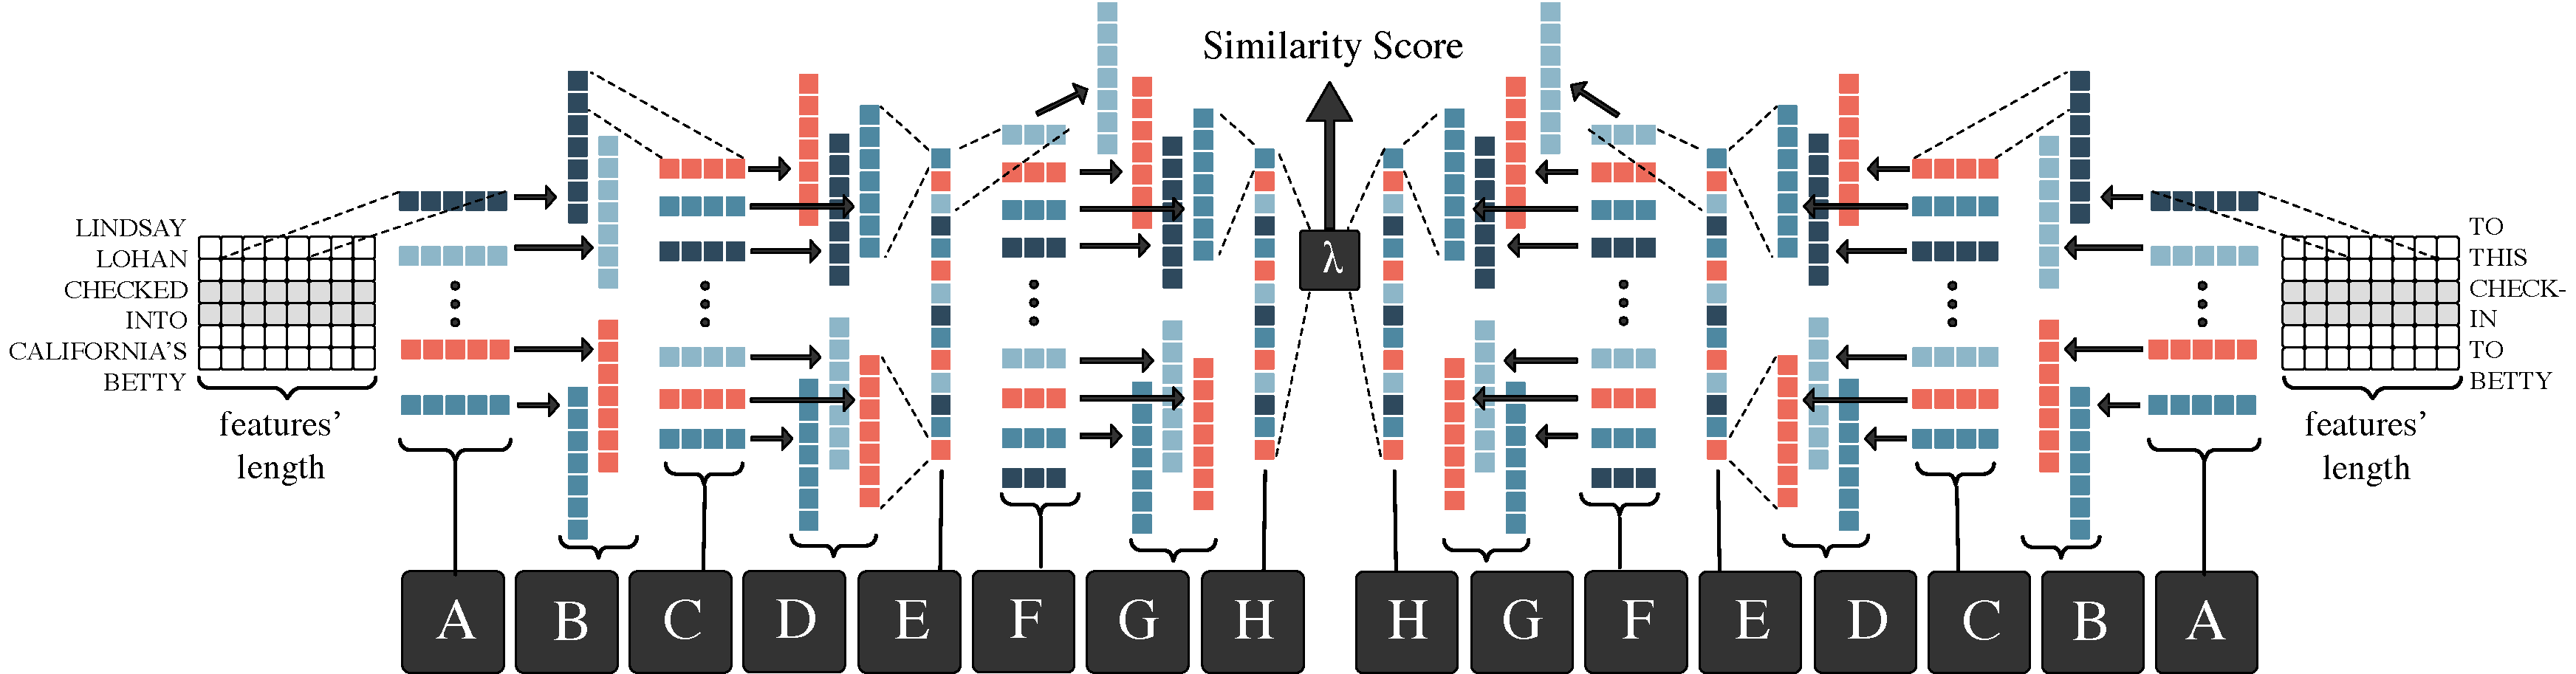
\includegraphics[width=1\textwidth]{architecture.pdf}
	\caption{Conjoined Convolutional Neural Network's Architecture.  The left half shares the same weights with the right half.  Blocks A, C, and F represent 32, 64, and 128 kernels, respectively.  The kernel size is 1x3, and different colors denote distinct kernels.  Blocks B, D, and G represent Convolution with stride of 1, ReLU activation, then 10\% dropout.  Blocks E and H represent MaxPooling with kernel size 1x2.  The Lambda function in the center represents the Euclidean Distance of the merged univariate vectors.}
	\label{fig:ccnn}
\end{figure*}

\subsection{Loss / Optimization}
Our goal is to maximize discriminability of different event mentions, while enforcing features to be as similar as possible when they are of the same event.  Contrastive Loss is perfectly suited for this objective \cite{SchroffKP15,pmlr-v48-liud16}, as shown in Equation \ref{eq:contrastive}. Our training set has a strong class imbalance (most input pairs are not co-referent), so we down-sample to a 5:1 ratio of negative-to-positive examples.  We use Adagrad for optimization.
\begin{equation}
\begin{aligned}
L(&\hat{y},y)=\frac{1}{2N}\sum_{n=1}^{N}[(y)d^2 \\
&\qquad {} + (1-y)*(max(1-d,0))^2] \\
&\textnormal{where }d=\|y_{n}-\hat{y}_{n}\|_{2}
\end{aligned}
\label{eq:contrastive}
\end{equation}

\section{Neural Clustering}
\label{sec:clustering}
It is common practice for mention-pair models to first assign a probability score to every mention-pair, and then cluster with a different model.

\subsection{Existing Clustering Approaches}
\textbf{Agglomerative Clustering} is a simple but effective approach.  It first assigns each mention to its own singleton cluster.  Then, it repeatedly merges the two distinct clusters which contain the shortest-distance mention pairs.  Although this is a strong baseline, as seen in Yang, et. al. \shortcite{journals/tacl/YangCF15}, there are three main weaknesses:
\begin{enumerate}
\item One must define a heuristic to stop merging.
\item If one uses a threshold value $\alpha$ to stop merging (i.e., merge while the shortest pair of mentions from distinct clusters is $<\alpha$), this relies on the data being uniform across documents. Yet, the distribution of pairwise predictions inevitable differs for each document, causing any given $\alpha$ to be appropriate for some documents but sub-optimal for others.
\item Most significant, each cluster merge is based solely on two individual mentions, yet these mentions may not be representative of the cluster at large.
\end{enumerate}

\textbf{HDDCRP and Iterative-Folding Clustering} both contain the issue \#3 above, as detailed in Sections \ref{sec:HDDCRP} and \ref{sec:Choubey}.

\subsection{Our Approach}
We aim to use the strengths of agglomerative clustering, while replacing its shortcomings.  We train a classifier to learn the most likely {positive cluster merge}, where the cluster is represented more holistically than a single pair.  Instead of operating on a mention-to-mention basis to dictate the cluster merges, we consider every possible mention-to-cluster.

Specifically, denoting a mention as $m$ and a cluster as $C$, we learn a function $f(m_i,C_y)$ that predicts the likelihood of an appropriate, positive merging of $(C_x,C_y)$, where $m_i \in C_x$ and $C_x \neq C_y$.

Let $d(m_i,m_j)$ be the mention-pair distance predicted by our CCNN model, where $m_i \in C_x$, and $m_j \in C_y$.  Function $f(m_i,C_y)$ is based on four simple features:
\begin{itemize}
  \item min-pair distance: $\min_{m_i,m_j} d(m_i,m_j)$
  \item avg-pair distance: $\frac{\sum_{m_j \in C_y} d(m_i,m_j)}{\|C_y\|}$
  \item max-pair distance: $\max_{m_i,m_j} d(m_i,m_j)$
  \item size of candidate cluster: $\|C_y\|$
\end{itemize}

The first three features serve to better represent the cluster at large.  For example, if a given $m_i$ were evaluated against two other clusters $C_1$ and $C_2$, it might be the case that both clusters of have the same min-pair distance score.  Yet, the \textit{distribution} of distance scores with the other mentions in each cluster might shed light onto which cluster has more similar mentions.  We experimented with including the full distribution of distance scores, along with the variance in distance scores, but we received the best results from the min, avg, max distances -- probably because most golden clusters contain just 1-4 mentions.  The last feature (cluster size) serves is an explicit measure to help prevent clusters from growing too large.

At testing time, we evaluate every $(m_i, C_y)$ pair.  

We define $f$ as a feed-forward neural network\footnote{We used 1 hidden layer of 25 units, ReLU activation without dropout, and Adagrad as our optimizer} which predicts the probability of a positive merge via a two-class softmax function.  Our loss function is weighted binary cross-entropy, to account for the class imbalance situation that most mentions should not be merged with most clusters.  In an easy-first manner, at each iteration, we merge only the $(m_i,C_y)$ pair that yielded the highest score (likelihood of a positive merge).  Then, we re-evaluate all (mention, cluster) pairs and repeat this process until the model no longer predicts any merge.  Thus, unlike the aforementioned models, we do not require an additional parameter for our stopping criterion.

Since our neural classifier requires as training data the mention-pair scores predicted by the CCNN, our model is limited to using the Dev Set's scores as training data.  We also considered (1) adjusting the Train/Dev set sizes, yielding more data on which our clustering model could train; and (2) cross-validation.  Yet, the original train/dev/test split performed the best, signifying that it is important for the CCNN model to have as much training data as possible, even at the expense of the Neural Clustering model having less training data.

\section{Results}
As a recap, our research concerns three independent axis of investigation:
\begin{itemize}
\item \textbf{Features:} which features are most useful, and can we use few features?
\item \textbf{Mention-Pair Model:} how well does CCNN perform against a standard feed-forward neural network\footnote{Given two mentions $i$ and $j$, with corresponding feature vectors $f_i$ and $f_j$, their input to the Feed-Forward Neural Network is the vector $\|f_{i} - f_{j}\|$} (FFNN)?
\item \textbf{Clustering:} can we outperform Agglomerative via our Neural Clustering model?
\end{itemize}

Our metric is CoNLL F1 score, which is a clustering-based metric that combines the F1 scores of MUC, $B^{3}$, and $CEAF_{e}$, and we use the official scorer script (v8.01) \cite{Pradhan+etal:14a}.

We were interested in the five common, non-relational embedding features which are detailed in Section \ref{sec:features}: POS, Lemma, Dependency Lemma, Character, Word.  We tested all combinations of features on the Dev Set, and Lemma yielded the best results (see Figure \ref{fig:allfeatures}).  Thus, our CCNN + Neural Clustering system used only the Lemma feature, and we evaluated it against other systems, as illustrated in Table \ref{tab:others}.  The results further show that our CCNN model outperforms a FFNN, and that our Neural Clustering outperforms Agglomerative Clustering.  Using just the lemma feature, we achieved a CoNLL F1 score of \textbf{81.2} on the ECB+ Test Set.  We denote this score as the new baseline to which to compare future systems.

\begin{figure*}[h]
\centering
	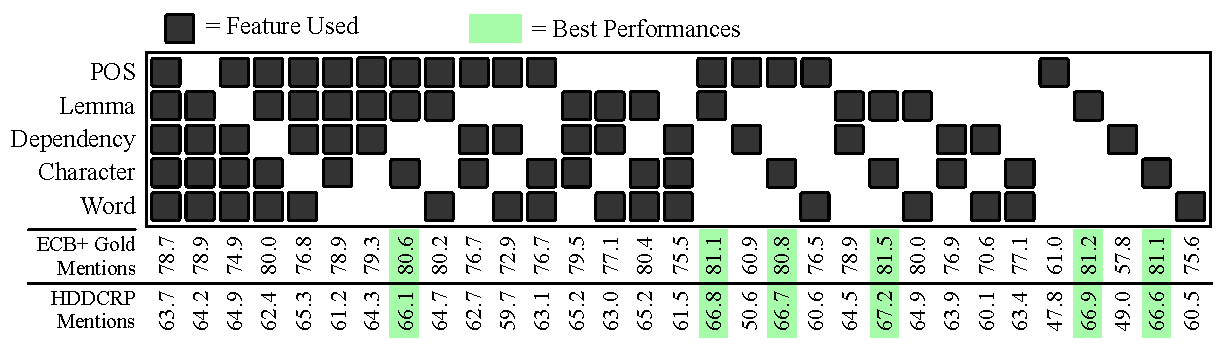
\includegraphics[width=0.82\textwidth]{features.pdf}
	\caption{The CoNLL F1 performance of our flagship CCNN + Neural Clustering system, using various features.  The CCNN mention-pair predictions for the Dev Set are normally used to train our Neural Clustering model.  So, in order to fairly evaluate our Neural Clustering on the \textit{Dev Set} Mentions, we removed Topics 18-20 from the CCNN's Training Set and used them to train our Neural Clustering.}
	\label{fig:allfeatures}
\end{figure*}

\begin{table}[h]
\centering
\tabcolsep=0.11cm
\begin{tabular}{|r|ccc|c|}
 \hline
 \multicolumn{5}{|c|}{Test Set: ECB+ Gold Test Mentions} \\
 \hline
& MUC & B$^3$ & CEAF & CoNLL F1\\
 \hline
 SameLemma& 58.3 & 83.0 & 75.9 & 72.4\\
FFNN+AGG & 59.9 & 85.6 & 78.4 & 74.6 \\
FFNN+NC & 60.7 & 86.7 &  79.4 & 75.6 \\
CCNN+AGG & 70.5 & 89.1 & 83.5  & 81.0\\
\textbf{CCNN+NC}  & 70.9 & 88.9 & 83.6 & \textbf{81.2} \\
\hline
\hline
 \multicolumn{5}{|c|}{Test Set: HDDCRP's Predicted Mentions} \\
 \hline
 SameLemma& 40.4 & 66.4 & 66.2 & 57.7\\
 HDDCRP & 53.4 & 75.4 & 71.7  & 66.8\\
 \textbf{CCNN+NC} & 53.7 & 75.2 & 71.9  & \textbf{66.9}\\
 \hline
\hline
 \multicolumn{5}{|c|}{Test Set: Choubey's et. al. Mentions} \\
 \hline
 SameLemma& 48.8 & 66.7 & 65.1 & 60.2\\
 Choubey & 62.6 & 72.4 & 71.8  & 68.9\\
 \textbf{CCNN+NC} & 67.3 & 73.0 & 69.5  & \textbf{69.9}\\
 \hline
\end{tabular}
\caption{Comparison against other systems, while our models use only the Lemma Embedding feature.  \textbf{Note:} CCNN+NC achieves even stronger results when using Lemma+Char features (\textbf{81.5, 67.2,} and \textbf{70.0} for the three sections, respectively). FFNN denotes a Feed-Forward Neural Network Mention-Pair model.  AGG denotes Agglomerative Clustering.  NC denotes our Neural Clustering model.}
\label{tab:others}
\end{table}

\textbf{Lemma Embeddings} were the most useful feature, followed closely by Character Embeddings.  Since \textit{SameLemma} has historically been a strong baseline, this is unsurprising.  Using the embeddings of the lemmas, especially with the power of the CCNN, provides much more expression than the mere boolean feature of \textit{SameLemma}.

\textbf{Character Embeddings} were effective for the same reason String Edit Distance is often a strong feature: there tends to be a direct correlation between the textual similarity of mentions and their likelihood of being co-referent. Both random character embeddings and pre-trained ones yielded the same performance, suggesting that the power comes from the uniqueness of characters, not any \textit{meaning} conveyed in the characters.

Combining Lemma + Character Embeddings gave even higher performance on all three Test Sets, illustrating that these two features are complementary; the semantic information conveyed within the lemma embeddings complement the syntactic information of character embeddings.  Related, POS by itself was a poor feature, but combining it with either Lemma or Character Embeddings offered strong results. 

Ideally, a classifier should precisely learn how to combine all features smartly, such that the unhelpful features are given no weight.  However, in practice, that is often extremely difficult, due to both the large parameter space and the high entropy wherein some combinations of features seem to equally help as much as hurt.  Thus, we conclude that one should try to use the fewest features as possible for coreference resolution, then to expand appropriately.

Interestingly, in all experiments, our results were inversely correlated with the amount of context our CCNN used.  That is, our best performance came when we used no context, only the mention words.  This agrees with the Choubey's, et. al. findings \shortcite{Choubey2017EventCR}.

\subsection{Comparison to Other Systems}
\textbf{HDDCRP} chose to not use the gold test mentions provided by ECB+.  Instead, they used a semantic role labeller to identify all test mentions.
To compare against their system, we worked with the HDDCRP source code and data to ensure we accurately use their same mentions.  Independent of clustering performance: of the 3,290 gold mentions in ECB+, their system failed to identify/use 676 of them.  Of their 3,109 predicted mentions, 495 were false positives and in fact not actual gold mentions.  Since their system uses these imperfect mentions, yet tests the coreference performance against the gold mentions, their system encounters a steep performance loss by default.  With complete confidence, we fairly compare our system with theirs by using the same, imperfectly-predicted mentions.  We outperform their system on this exact test set, as shown in Table \ref{tab:others}.

\textbf{Iteratively-Unfolding} attempted to use the same predicted test mentions as HDDCRP.  However, their test set actually differed, as detailed in Section \ref{sec:mentionid}.  We compare against theirs in Table \ref{tab:others}.

For event within-doc coreference, our system outperforms both HDDCRP and Iteratively-Unfolding.  Notably, both systems also perform cross-document coreference in a manner that helps inform and improve their within-doc performance; yet, we demonstrate state-of-the-art results without using this process.

\section{Conclusion}
In summary, we researched within-doc event coreference resolution, and our approach was novel by using a Conjoined Convolutional Neural Network as a mention-pair model, followed by a neural clustering model.  Unlike most coreference systems which rely on dozens of features, we used only lemmatization and pre-trained word/character embeddings.  We illustrate the performance of five commonly used features, demonstrating the effectiveness of using few features.  Our Neural Clustering model addressed a common weakness in mention-pair models: instead of forming clusters based on just \textit{one} pair of mentions satisfying a criterion, we used simple mention-cluster features which represent clusters more holistically.  Our system achieved state-of-the-art performance of 66.9 CoNLL F1 on a common test set, and we set a new baseline of 81.2 CoNLL F1 for the entire ECB+ test set.   

% include your own bib file like this:
%\bibliographystyle{acl}
%\bibliography{naaclhlt2018}
\bibliography{naaclhlt2018}
\bibliographystyle{acl_natbib}
\end{document}
